% -*- mode: noweb; noweb-default-code-mode: R-mode; -*-











\graphicspath{ {analysis/} }

\chapter{Analysis}
\label{cha:analysis}




In this chapter we will describe a procedure for combining information
from the data sets described in \autoref{cha:datasets} using the same
sub-pixel analysis data structure at $5'$ resolution for the
conterminous USA9 (cUSA) to produce a data set that exhibits high
accuracy in the distribution of agricultural production according to
the Agland2000 data set introduced in \autoref{sec:agland2000}, that
provides a realistic characterization of other uses and covers as
suggested by MLCT data from \autoref{sec:mlct} and particular aspects
of the NLCD from \autoref{sec:nlcd}.

In this chapter we will evaluate the progress of the analysis in terms
of areas given both in millions of acres (Ma) and millions of hectare
(Mha).  It is important to note that these areas cannot be computed
directly from the geographic grid in which the data is contained and
our maps are rendered.  Because these $5'$ grid cells are actually
sections of a spheroid projected onto a plane, the areas that a given
cell encompasses is not constant.  A first-order approximation of
these areas can be obtained as a function of the earth's mean radius
and the cosine of a cell's latitude.  In this way areas are maximum at
the equator and approach zero as position approaches the poles.
Conveniently Hijmans' \texttt{raster} package for the \texttt{R}
analysis software provides a function \texttt{area()} that accepts any
raster data set in geographical coordinates (longitude, latitude) as
an input, producing a new raster data set whose values are the areas
of the former in km$^{\textrm{2}}$.  It is a simple matter to convert these to
acres by subsequently scaling that result by a constant.  See the
source code in the appendix for further details.

We start by tabulating the aggregate areas by PEEL class for the data
sets that we are using as inputs, MLCT, NLCD, and Agland2000.  We
evaluate the accuracy of cropland distribution in the MLCT data as a
function of two values of the $A_{min}$ parameter, which is defined as
the minimum fraction of an MLCT pixel at its native resolution
assigned to the primary class prior to aggregation to the $5'$ PEEL
model analysis grid.  $A_{min}=1.0$ represents consideration of only
the primary class.  $A_{min}=0.5$ indicates that in the hypothetical
situation of zero classification confidence the primary class would be
assigned half of the area of that particular MLCT pixel, therefore
this value represents maximum incorporation of the secondary class in
our analytical framework, as modulated by the MLCT classification
confidence data.  These intermediate results are compared on the basis
of root mean squared error (RMSE) metrics calculated relative to the
distribution of cropland given in the Agland2000 data at the end of
\autoref{sec:comparison}.

In \autoref{sec:nlcd_offsets} we describe a method for selectively
incorporating cover fractions for particular classes from the NLCD
data set due to a perceived underestimation of those classes by MLCT
due primarily to its lower resolution.  Those classes are water,
wetland, and urban.  In the PEEL classification the ``urban'' class is
broadened to include rural infrastructure that MLCT effectively counts
as cropland.  Accepting NLCD's quantification of these classes as
truth is intended to counteract a perceived overestimation of cropland
area in MLCT caused in part by a discrepancy in formulation of these
data sets, Agland2000 representing actual harvested areas and MLCT
catching up lots of ancillary land that may be associated with
cultivated land but is not directly involved in crop production. The
result is an adjusted version of the MLCT data as amended by these
NLCD offsets.

Section~\ref{sec:fusion} presents the results of fusing our adjusted MLCT
map with the Agland2000 data by accepting the Agland2000 value for
cropland as truth where possible and scaling other classes
proportionally to describe the remainder of the landscape for
purposes of the PEEL model.  This operation is constrained by our
decision to retain the NLCD offsets as firm figures for those classes
in order to account for varying degrees of infrastructure development
represented by the so-called urban class and water or wetland features
not resolved in the MLCT data.  Where Agland2000 conflicts with this
constraint the cropland fraction is reduced accordingly.

Finally \autoref{sec:peel} shows how information from the
\texttt{175Crops2000} data set is used to disaggregate the cropland
given by the result of the previous step in order to provide a rough
characterization of the distribution of production of major crop
commodities, corn (maize), soybean, wheat, rice, sugarcane, other
cereals, and other field crops.  This is important for the PEEL model
because the intent is to model transitions in production in response
to forecast commodity prices in addition to other drivers.

Through the offset and fusion steps we use decreasing RMSE figures to
show that our complete characterization of the landscape is improving
in accuracy with respect to \texttt{Agland2000}, the census-based
distribution of productive cropland so that when other cover classes
are scaled the distortions are minimized.


\section{Comparison of Aggregate Areas}
\label{sec:comparison}


% latex table generated in R 2.13.0 by xtable 1.5-6 package
% Fri Jul 22 17:34:06 2011
\begin{table}[ht]
\begin{center}
{\small
\begin{tabular}{rrrrrrr}
  \hline
 & Agland2000 & NLCD & \pbox[c][][c]{3in}{Aggregated\\$A_{min}=0.5$} & \pbox[c][][c]{3in}{Aggregated\\$A_{min}=1.0$} & \pbox[c][][c]{3in}{No Mosaic\\$A_{min}=0.5$} & \smallskip\pbox[c][][c]{3in}{No Mosaic\\$A_{min}=1.0$} \\ 
  \noalign{\smallskip} \hline
crop & 446.5 & 310.8 & 378.9 & 369.6 & 495.4 & 488.1 \\ 
  open & 557.1 & 429.6 & 516.9 & 545.8 & 538.7 & 561.9 \\ 
  forest & 0.0 & 513.2 & 344.7 & 353.6 & 410.8 & 429.9 \\ 
  shrub & 0.0 & 420.1 & 358.7 & 341.8 & 387.2 & 368.0 \\ 
  barren & 0.0 & 24.5 & 32.8 & 28.9 & 32.8 & 28.9 \\ 
  urban & 0.0 & 102.8 & 27.3 & 29.8 & 27.3 & 29.8 \\ 
  wetland & 0.0 & 95.0 & 26.0 & 11.0 & 26.0 & 11.0 \\ 
  water & 0.0 & 96.5 & 74.3 & 75.0 & 74.3 & 75.0 \\ 
  mosaic & 0.0 & 0.0 & 232.9 & 237.0 & 0.0 & 0.0 \\ 
  total & 1003.7 & 1992.5 & 1992.5 & 1992.5 & 1992.5 & 1992.5 \\ 
   \noalign{\smallskip} \hline
\end{tabular}
}
\caption{Total Acreages by Map and Cover}
\label{tab:areas}
\end{center}
\end{table}
\begin{figure}[ht] 
  \centering


  \includegraphics{fig_areas}
  \caption{Total Acreages by Map and Cover}
  \label{fig:areas} 
\end{figure} 


After decomposing the mosaic class MLCT indicates
495.4 Ma ( 200.5 Mha) of cropland for
$A_{min}=0.5$ and 488.1 Ma ( 197.5 Mha) for
$A_{min}=1.0$ in the cUSA in 2001.  Aglands2000 indicates roughly
446.5 Ma ( 180.7 Mha) of cropland.  The
inability of the MLCT data set to resolve rural transportation
networks, minor settlements, and small water or wetland features is a
major contribution to the surplus of cropland acreage indicated by the
MLCT.  Due to its greater resolution, ~30m vs. ~500m, the NLCD is
better suited at discerning developed areas in rural landscapes
ranging from rural roads to farmsteads to small communities that do
not show up in the MLCT data. There is a total area of roughly
75.4 Ma ( 30.5 Mha)
of development remaining after subtracting the MLCT urban class from
all developed classes in the NLCD after they have both been aggregated
to the $5'$ grid. Applying this area as an offset to the cropland
area in Aglands2000 brings us closer to the expected acreage under
cultivation in 2001, although this assumes that all of that
development intersects with MLCT cropland area.

The purpose for processing the MLCT for two values of $A_{min}$ as
described in \autoref{cha:datasets} was to evaluate whether or not
information from the secondary cover type contributes positively to
the accuracy of the data set we seek to synthesize.  The primary
objective of this synthesis is to achieve accuracy in cropland
distribution.  Because the cropland layer in the Agland2000 data set
is derived from county-level production census statistics we adopt
this as the ground truth and will endeavor to adjust our product
accordingly.  Although MLCT overstates cropland acreage for both
$A_{min}=0.5$ and $A_{min}=1.0$ the discrimination among the two is made
by the distribution of errors rather than the aggregate error.


\begin{figure}[ht] 
  \centering


  \includegraphics{fig_nomosDiff1}
  \caption{Difference between MLCT (no mosaic, $A_{min}=1.0$) and Agland2000 crop}
  \label{fig:nomosDiff1} 
\end{figure} 

\begin{figure}[ht] 
  \centering


  \includegraphics{fig_nomosDiff05}
  \caption{Difference between MLCT (no mosaic, $A_{min}=0.5$) and Agland2000 crop}
  \label{fig:nomosDiff05} 
\end{figure} 

\autoref{fig:nomosDiff1} and \autoref{fig:nomosDiff05} show the
cell-by-cell differences between the MLCT-derived data set that we
have calculated after mosaic decomposition and the Agland2000 cropland
map.  To summarize and compare these errors we calculate the root of
the mean squared error (RMSE) given by:

$$
\operatorname{RMSE}=\sqrt{\frac{\sum_{i=1}^{n}(\hat\theta_i-\theta_i )^2}{n}}
$$

where $\hat\theta_i$ are the predictions derived from the respective
MLCT derivations and $\theta_i$ are the observations taken from the
Agland2000 data set.




\begin{figure}[ht]
  \centering


\includegraphics{fig_hexPlot1}
  \caption{Hexbin plot of MLCT crop ($A_{min}=1.0$, no mosaic) versus Agland2000 cropland}
  \label{fig:hexplot1} 
\end{figure} 

To examine the relationships between the distributions of cropland
that we derive from the MLCT data relative to the Agland2000 data we
will use ``hexbin'' plots which are essentially two-dimensional
histograms that show the number of grid cells that occur within
discrete regions of the space defined by coordinates that are cropland
fractions for the two data sets.  This operates much like a common
scatter plot but for data sets with as many observations as we wish to
include it gives a cleaner representation of that structure.  For our
plots we have chosen to employ a logarithmic scale because of the wide
range of counts calculated for the bins.  This gives a more complete
picture of the overall dispersion and local concentration of the
observations.  Our first example of such a plot is
\autoref{fig:hexplot1} which plots the crop fractions of MLCT with
$A_{min}=1$ versus those of the Agland2000 crop map.  As one would
expect there is an overall correlation among these variables,
especially given that Agland2000 provides prior probabilities to the
MLCT classification.  It is clear that the MLCT primary class
exhibits a positive bias overall, although a subset that is negatively
biased is also apparent for low values of the Agland2000 crop fraction
in the interval $[0.1,0.5]$.  Also of particular note is the drastic
decrease in correlation when Aglands2000 reaches 1.0 relative to the
stronger relationship over the interval $[0.8,1.0)$.  It is difficult
to speculate on the nature of this structure, but suffice it to say
that there is something peculiar about the Agland2000 allocation
procedure that drives the crop fraction to its maximum in areas where
the remote sensing data clearly resists such a characterization.  This
may be caused by systematic errors in the agricultural census data
that drive the Agland2000 algorithm forcing unrealistically high
concentrations in order to satisfy the algorithm's constraints. 
 



\begin{figure}[ht]
  \centering



\includegraphics{fig_hexPlot05}
  \caption{Hexbin plot of MLCT crop ($A_{min}=0.5$, no mosaic) versus Agland2000 cropland}
  \label{fig:hexplot05} 
\end{figure} 

% latex table generated in R 2.13.0 by xtable 1.5-6 package
% Fri Jul 22 17:34:29 2011
\begin{table}[ht]
\begin{center}
\begin{tabular}{rr}
  \hline
$A_{min}$ & RMSE \\ 
  \hline
0.5 & 0.165 \\ 
  1.0 & 0.180 \\ 
   \hline
\end{tabular}
\caption{RMSE, MLCT vs. Agland2000 crop}
\label{tab:rmse}
\end{center}
\end{table}
\todo{Consider also calculating statistical bias (average error)?}

We expect that setting $A_{min}=1$ will produce a maximum overall bias
and attendant error by assigning entire pixels to the cropland class
and not allowing for the possibility of mixed covers.  The results on
\autoref{tab:rmse} indicate that $A_{min}=0.5$ is more representative
of the distribution of cropland because although the total area
indicated is higher according to \autoref{tab:areas}, there is less
error on a cell-by-cell basis indicating that it does a better job of
representing the spatial distribution than $A_{min}=1.0$.  This is
reflected in the structure revealed by \autoref{fig:hexplot05} where
fewer cells in the MLCT data are set at 100\% crop because of
including the secondary class in calculating $5'$ coverage fractions.
Where crop was included in a secondary class it also caused cells of
near-zero value for MLCT to lift away from the x-axis.  The
uncorrelated observations for Agland2000 equal to 1.0 are still
present, however.  This result is adequate for our purposes to
determine that our logic in considering the secondary class in the
manner we have for $A_{min}=0.5$ is correct.  From this point forward
we will consider only the statistics derived from setting
$A_{min}=0.5$ for the aggregation of the MLCT data due to this
improved fit with Agland2000 cropland and its full consideration of
all information imparted by the MLCT data.


\section{NLCD Offsets}
\label{sec:nlcd_offsets}


From \autoref{tab:areas} it is apparent that the MLCT results are
negatively biased in the total areas assigned to water, wetland, and
urban features relative to the NLCD.  It is clear from visual
inspection that features of these classes tend to have smaller
characteristic dimensions which causes them to be overlooked in the
MLCT data due to its resolution.  The most obvious example is the
rural transportation networks in areas surveyed under the Public Land
Survey System (PLSS) where roads have been laid out on a generally
regular grid of square miles.  In the PEEL classification this
infrastructure is included in the urban class as another form of
developed land, perhaps making ``urban'' somewhat of a misnomer, but
it hails to its origins in the IGBP classification scheme and provides
a short label, a great convenience in programming.  It is important to
represent wetlands and water features in our input to the PEEL model
because these areas have high likelihoods of being set aside for
conservation purposes, which would be represented as a constraint on
land conversion in the model.  In the event that NLCD overestimates
these areas it would be an acceptable error to carry over to the PEEL
model in order to be conservative in allowing for conservation
measures in a greater number of grid cells, absent more precise LULC
data with respect to the water and wetland classes.

To merge this information from the NLCD we begin by simply accepting
the areas for water, wetland, and urban classes in the reclassified,
$5'$-aggregated version of NLCD that we have computed as truth and
calculate offsets for those classes versus our $5'$ MLCT data by
straight subtraction.  Where NLCD is greater the difference will be
positive and so a positive offset will be added to the fraction
already present for any one of the ``truth'' classes from NLCD.  The
other classes are then adjusted so that they are present in proportion
to each other as indicated by MLCT but in the area remaining after
accepting the water, wetland, and urban areas from NLCD.  The additive
offsets needed to achieve this balance and account for the entire area
of the cell are calculated so that the effects of this process on all
classes may be considered on a common basis.  

For the calculation of the offsets we drop back to the result of
aggregating the MLCT data to $5'$ with $A_{min}=0.5$ prior to mosaic
decomposition.  Presumably there are rural roads comprised of 30m NLCD
pixels cutting through the lower-resolution MLCT pixels including
those classified as mosaic.  In fact, by its very nature as a hybrid
class made up of natural cover and agricultural land use we expect
roads to be an important component of the landscape.
\autoref{fig:offsets1} and \autoref{fig:offsets2} show the spatial
distributions of the offsets calculated based on our assumptions about
the water, wetland, and urban classes in the NLCD.  We have verified
that these offsets sum to zero for each grid cell.  Any area deducted
from one class must be added to one or more classes in the same cell
in order to conserve the total area and maintain the sum of the
fractions at 1.0.


\begin{figure}[h]
  \centering


\includegraphics{fig_offsets1}
  \caption{NLCD offsets}
  \label{fig:offsets1} 
\end{figure} 


\begin{figure}[h]
  \centering


\includegraphics{fig_offsets2}
  \caption{NLCD offsets (cont.)}
  \label{fig:offsets2} 
\end{figure} 


The maps of these offsets are shown using a logarithmic scale in
order to bring attention both to areas of significant adjustment,
greater than 10\%, as well as to show the extent to which small
adjustments on the order of 1--5\% occur.  From these maps we can see
the detailed structure of drainage networks in the water class and
population centers in the urban class which could easily be confused
with the vegetative classes in the MLCT classification.  This refers,
for example, to heavily wooded suburbs where transportation
infrastructure is obscured and difficult to resolve.  The offsets for
the NLCD truth classes are generally positive, although not strictly
so because the algorithm does not preclude the possibility that MLCT
may locally overestimate these classes in particular regions and still
suffer an aggregate deficit relative to NLCD.


\begin{figure}[ht]
  \centering
    \includegraphics{fig_corOffsets}
  \caption{Correlation matrix of NLCD offsets}
  \label{fig:corOffsets} 
\end{figure} 

\autoref{fig:corOffsets} shows the result of calculating a matrix of
correlations among the offsets calculated for each class based on
NLCD.  Each cell in the matrix reflects the value of the statistical
correlation between the corresponding classes within the NLCD offset
maps resulting from the algorithm described above.  This gives us an
overall sense of the effect of applying these offsets by showing which
changes are strongly correlated, whether it be positively or
negatively.  It is a symmetric matrix because the classes on both axes
are from the same data set and any single classes is, of course,
perfectly correlated with itself.  Going in we would expect to see
negative correlations between classes accepted as truth from NLCD,
water, wetland, and urban, and the other classes because the purpose
of applying these offsets was to bring the total areas of these
classes up, which can only happen at the expense of the other classes.
For example the wetland offsets show strong negative correlations with
forest, shrub, and mosaic.  This stands to reason as a likely problem
with classification due to fundamental differences in the remote
sensing data such as resolution, the interpretation thereof, or
disagreement/overlap in class definitions.  Many areas of forest
and shrub land can exhibit properties of a wetland when standing water
and high soil moisture are persistent.  The ``NLCD truth'' classes'
offsets are positively correlated with one another because they are
generally positive everywhere.  Likewise, non-truth classes are
positively correlated with one another because they are all being
assigned negative offsets to make room for the increased values of
water, wetland, and urban fractions.  The crop and mosaic classes are
most strongly negatively correlated with urban which reflects the
widespread adjustments to account for rural transportation networks
and smaller settlements.

The resulting offsets are added to the aggregated fractions calculated
from the MLCT with $A_{min}=0.5$.  The mosaic decomposition step is
readily applied to the adjusted data set because the adjusted
fractions are fundamentally in same form as the intermediate form of
the MLCT data calculated in \autoref{sec:decomposition}, only the
values have changed.














To assess whether the process of adding in the NLCD offsets has
improved overall cropland accuracy we can perform the same error
calculation from above and extend Table~\ref{tab:rmse} with the new
result, giving us Table~\ref{tab:rmse2}.

% latex table generated in R 2.13.0 by xtable 1.5-6 package
% Fri Jul 22 17:37:36 2011
\begin{table}[ht]
\begin{center}
\begin{tabular}{lrr}
  \hline
offset & $A_{min}$ & RMSE \\ 
  \hline
TRUE & 0.5 & 0.151 \\ 
  FALSE & 0.5 & 0.165 \\ 
  FALSE & 1.0 & 0.180 \\ 
   \hline
\end{tabular}
\caption{RMSE, MLCT vs. Agland2000 crop with NLCD offsets}
\label{tab:rmse2}
\end{center}
\end{table}
% \todo[caption=Should the RMSE tables be rearranged?]{Would it make
%   more sense to have the row order and independent variables (first
%   three) reversed in Table \ref{tab:rmse} and \ref{tab:rmse2}?}

% \todo[caption=Should references to the pasture/open data from
% Aglands2000 be removed?]{That data is not used in the analysis,
%   although it is interesting to see that it's RMSE declines as well.}

Seeing that this modification to the data set has improved our overall
accuracy of the distribution of croplands the next step is to examine
the total areas for all classes compared with the input data sets.  


% latex table generated in R 2.13.0 by xtable 1.5-6 package
% Fri Jul 22 17:37:36 2011
\begin{table}[ht]
\begin{center}
{\small
\begin{tabular}{rrrrrrrr}
  \hline
 & Agland2000 & NLCD & MLCT & \pbox[c][][c]{3in}{MLCT\\No Mosaic} & \pbox[c][][c]{3in}{NLCD\\Offsets} & \pbox[c][][c]{3in}{MLCT\\Adjusted} & \pbox[c][][c]{3in}{\smallskip{}MLCT\\Adjusted\\No Mosaic} \\ 
  \noalign{\smallskip} \hline
water & 0.0 & 96.5 & 74.3 & 74.3 & 22.3 & 96.5 & 96.5 \\ 
  forest & 0.0 & 513.2 & 344.7 & 410.8 & -44.7 & 300.1 & 355.7 \\ 
  shrub & 0.0 & 420.1 & 358.7 & 387.2 & -23.8 & 334.9 & 358.0 \\ 
  open & 557.1 & 429.6 & 516.9 & 538.7 & -21.0 & 495.9 & 514.9 \\ 
  wetland & 0.0 & 95.0 & 26.0 & 26.0 & 69.0 & 95.0 & 95.0 \\ 
  crop & 446.5 & 310.8 & 378.9 & 495.4 & -39.0 & 339.9 & 437.6 \\ 
  urban & 0.0 & 102.8 & 27.3 & 27.3 & 75.4 & 102.8 & 102.8 \\ 
  mosaic & 0.0 & 0.0 & 232.9 & 0.0 & -37.4 & 195.5 & 0.0 \\ 
  barren & 0.0 & 24.5 & 32.8 & 32.8 & -0.9 & 31.9 & 31.9 \\ 
  (all) & 1003.7 & 1992.5 & 1992.5 & 1992.5 & -0.0 & 1992.5 & 1992.5 \\ 
   \noalign{\smallskip} \hline
\end{tabular}
}
\caption{Effect of NLCD offsets on total acreages, $A_{min}=0.5$}
\label{tab:areas2}
\end{center}
\end{table}

\begin{figure}[ht]
  \centering


  \includegraphics{fig_offsets}
  \caption{Total offsets calculated from NLCD}
  \label{fig:offsets}
\end{figure}


\autoref{fig:offsets} shows the totals by class of the offsets that
result from this calculation.  The item labeled ``total'' appears
blank because a value of zero is plotted there indicating that area
was conserved in this operation, which is to sat that area subtracted
from one class was reallocated to another.  As expected, the most
significant offset was for the urban class, representing the
low-density infrastructure outside of concentrations of development
large enough and dense enough to be identified in the MLCT
classification.  Water and wetland fractions were also increased to
bring the total areas of those classes in line with NLCD.  However,
the most important outcome with respect to our stated objective of
bringing total cropland areas in line with the total from Aglands2000
is the reduction of crop areas by
39 Ma ( 15.8 Mha) and mosaic areas
by 37.4 Ma ( 15.2 Mha).  This will
result in a total reduction of
57.8 Ma ( 23.4 Mha)
of the final crop class after mosaic decomposition because mosaic land
is taken to be half cropland by definition.  \autoref{fig:areasAdj}
shows the effect of adding these offsets and subsequently performing
the mosaic decomposition operation, which brings the cropland area for
the PEEL input data set into closer agreement with Aglands2000,
437.6 Ma ( 177.1 Mha) and
446.5 Ma ( 180.7 Mha) respectively. The
significance of this result is that it is in no way conditioned by the
desired cropland area estimate, rather shows a convergence in these
estimates by selectively incorporating information about other classes
from an independent data set, namely NLCD.

\begin{figure}[ht]
  \centering


  \includegraphics{fig_areasAdj}
  \caption{Total acreages after NLCD adjustment}
  \label{fig:areasAdj}
\end{figure}


\begin{figure}[ht] 
  \centering

    \includegraphics{fig_hexPlotAdj}
  \caption{Hexbin plot of MLCT adjusted crop versus Agland2000 cropland}
  \label{fig:hexPlotAdj} 
\end{figure} 


\section{Fusion of Adjusted MLCT and Agland2000}
\label{sec:fusion}



By bringing the aggregate crop areas of our MLCT-derived data set into
greater agreement with Agland2000 and accepting the water, wetland,
and urban fractions indicated by the NLCD we are now ready for the
final manipulation of the remaining classes, forest, shrub, open, and
barren, that will bring our complete data set into maximum agreement
with Agland2000.  To do this we will be setting the crop fraction
equal to Agland2000's crop value everywhere that this does not
conflict with the allocation indicated by the NLCD offsets.  Anywhere
that there is a conflict such that Agland2000 indicated more cropland
than allowed by the NLCD offsets the crop fraction will be set to one
minus the total of the offsets and all other classes will be set to
zero.  Otherwise the non-offset, non-crop classes will be scaled to
fit proportionally into the remaining area left after incorporating
those classes which we have given primacy.  The assumption in this step
is that the census data behind the Agland2000 crop map is a ``ground
truth'' and Ramankutty's method for allocating that area within the
$5'$ grid is sufficiently faithful to that truth.  The one difficulty
of note in this step is the presence of cells where we have
MLCT/NLCD-derived fractions for LULC but Agland2000 is null, that is
to say that no data is given indicating that those cells were not
included in the land mass.  In those cases we accept the crop fraction
previously calculated since there is nothing to compare it against.


\begin{figure}[ht] 
  \centering


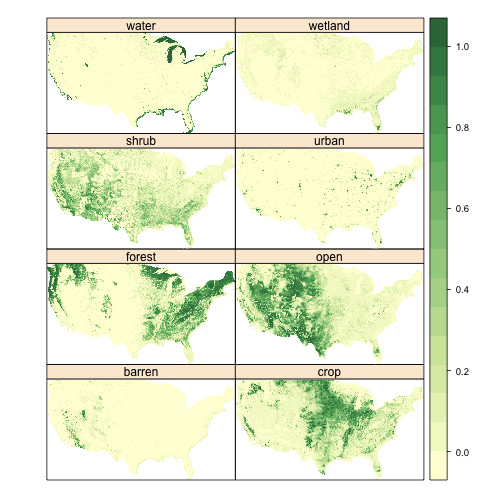
\includegraphics{fig_agc}
\caption{Final PEEL maps} 
\label{fig:agc} 
\end{figure} 

\begin{figure}[ht] 
  \centering


\includegraphics{fig_agc2}
\caption{Final PEEL cover maps (cont.)} 
\label{fig:agc2} 
\end{figure} 




% latex table generated in R 2.13.0 by xtable 1.5-6 package
% Fri Jul 22 17:38:49 2011
\begin{table}[ht]
\begin{center}
\begin{tabular}{llrr}
  \hline
agland & offset & $A_{min}$ & RMSE \\ 
  \hline
TRUE & TRUE & 0.5 & 0.017 \\ 
  FALSE & TRUE & 0.5 & 0.151 \\ 
  FALSE & FALSE & 0.5 & 0.165 \\ 
  FALSE & FALSE & 1.0 & 0.180 \\ 
   \hline
\end{tabular}
\caption{RMSE of PEEL vs. Agland2000}
\label{tab:rmse3}
\end{center}
\end{table}
% latex table generated in R 2.13.0 by xtable 1.5-6 package
% Fri Jul 22 17:38:56 2011
\begin{table}[ht]
\begin{center}
{\small
\begin{tabular}{rrrrrr}
  \hline
 & Agland2000 & NLCD & \pbox[c][][c]{3in}{MLCT\\No Mosaic} & \pbox[c][][c]{3in}{\smallskip{}MLCT\\Adjusted\\No Mosaic} & PEEL \\ 
  \noalign{\smallskip} \hline
water & 0.0 & 96.5 & 74.3 & 96.5 & 96.6 \\ 
  forest & 0.0 & 513.2 & 410.8 & 355.7 & 380.9 \\ 
  shrub & 0.0 & 420.1 & 387.2 & 358.0 & 362.8 \\ 
  open & 557.1 & 429.6 & 538.7 & 514.9 & 479.1 \\ 
  wetland & 0.0 & 95.0 & 26.0 & 95.0 & 95.0 \\ 
  crop & 446.5 & 310.8 & 495.4 & 437.6 & 443.7 \\ 
  urban & 0.0 & 102.8 & 27.3 & 102.8 & 102.8 \\ 
  mosaic & 0.0 & 0.0 & 0.0 & 0.0 & 0.0 \\ 
  barren & 0.0 & 24.5 & 32.8 & 31.9 & 31.7 \\ 
  (all) & 1003.7 & 1992.5 & 1992.5 & 1992.5 & 1992.5 \\ 
   \noalign{\smallskip} \hline
\end{tabular}
}
\caption{PEEL acreages, $A_{min}=0.5$}
\label{tab:areas3}
\end{center}
\end{table}
\todo{Discuss implications of final area tabulation}
 

\begin{figure}[ht] 
  \centering

    \includegraphics{fig_hexPlotAgc}
  \caption{Hexbin plot of PEEL crop versus Agland2000 crop}
  \label{fig:hexPlotAgc} 
\end{figure} 



\begin{sidewaysfigure}[ht] 
  \centering


    \includegraphics{fig_agcThemeMap}
  \caption{Conflicts between NLCD offsets and Agland2000}
  \label{fig:agcThemeMap} 
\end{sidewaysfigure} 


\autoref{fig:agcThemeMap} shows a thematic map that classifies the
cells in our study area according to their agreement on the cropland
fraction between Ramankutty's Agland2000 data set and the newly
created PEEL data set.  The first class indicated by ``PEEL = 0'' in
the legend represents where Agland2000 cropland fraction is zero so
there is no potential for conflict.  The second class shows where the
PEEL crop fraction is greater than zero but Agland2000 is null,
meaning no data was given for those cells.  Such cells generally occur
in coastal areas and on the shores of the Great Lakes, reflecting that
Rmankutty's criteria for counting a cell as ``dry land'' was somehow
more restrictive.  The third class shows where the NLCD ``truth''
classes (water, wetland, urban) allowed us to bring the PEEL crop
fraction in line with Agland2000 without violating the assumption that
those fractions should be carried over from the NLCD aggregation.  The
fourth class reveals where those constraints could not be
simultaneously satisfied.  Those cells correspond to the bins in
\autoref{fig:hexPlotAgc} that fall below the equality line because the
values from the NLCD offsets are given precedence and the crop
fraction is limited accordingly, which of course might mean that other
non-offset, non-crop classes could be summarily reduced to zero.  The
final class highlights pixels that Agland2000 assigns a crop fraction
of 1.0 which seems unrealistic given that some infrastructure and
uncultivated cover must be present within such large areas.

\section{Disaggregation of PEEL Crop Fractions According to 175Crops2000}
\label{sec:peel}





\begin{figure}[ht] 
  \centering

    \includegraphics{fig_cropSubClassesMap}
  \caption{Normalized fractions for crop sub-classes}
  \label{fig:cropSubClassesMap} 
\end{figure} 

\begin{figure}[ht] 
  \centering

    \includegraphics{fig_cropSubClassesMap2}
  \caption{Normalized fractions for crop sub-classes (cont.)}
  \label{fig:cropSubClassesMap2} 
\end{figure} 


We could assume that forage crops come from open class but we don't
know enough about the confusion between Aglands2000 pasture and the
open class in the first place, much less to make an informed
speculation about how forage crops would be classified by MLCT.  The
focus here is field crops so that is the only class that we are
attempting to disaggregate and forage crops are included there for
now.  Tree and shrub crops could be taken from the corresponding cover
types, but assuming that they are caught up in that classification is
a blind leap and their areas are small.  On the other hand, their
economic impact may be disproportionate to their areas by virtue of
price, but this will have to be studied more carefully.

Double-cropping is ignored for now by normalizing the crop fractions
by the sum of all crops, which can exceed unity in instances of
intense double-cropping.  The predominant double-cropping system in
the cUSA to our knowledge is soy followed by winter wheat, but there
may be others such as multiple cropping of rice in the southern
extremes of its range.  In areas where soy and wheat are
double-cropped their areas will be underestimated in this data set
relative to that given in the 175Crops2000 data set, subsequent to the
NLCD offset adjustment.  This issues also bears further study.




%%% Local Variables: 
%%% mode: latex
%%% TeX-master: "thesis"
%%% End: 

